
\documentclass[sigconf]{acmart}
\usepackage[T1]{fontenc}
\usepackage[utf8]{inputenc}

\usepackage{wrapfig} 
\usepackage{lmodern}
\usepackage{booktabs} %
\graphicspath{{figures/}}
\DeclareGraphicsExtensions{.pdf,.PDF,.png,.PNG}  

\usepackage{csquotes}
\usepackage{xcolor}
\usepackage{balance}
\usepackage{siunitx}
\usepackage{csquotes}
\usepackage{gensymb}
\usepackage{enumitem}
 
\definecolor{cardinal}{rgb}{0.77, 0.12, 0.23}
\newcommand{\redify}[1]{\textcolor{cardinal}{#1}}
\definecolor{cobalt}{rgb}{0.0, 0.28, 0.67}
\newcommand{\blueify}[1]{\textcolor{cobalt}{#1}}

\acmArticle{4}
\acmPrice{15.00}

\usepackage{eso-pic}
\AddToShipoutPictureFG{\AtPageLowerLeft{\put(\LenToUnit{0.5\paperwidth},\LenToUnit{6mm}){\makebox[0pt][c]{\fontsize{6.5}{8}\selectfont\color{gray}Author's revised version (2026-11-12). Version of record: \url{https://doi.org/10.1145/3231622.3231638}}}}}
\begin{document}
\title{Interactive, Height-based Filtering in 2.5D Treemaps}

\author{Daniel Limberger}
\orcid{0000-0002-9111-4809}
\affiliation{%
\institution{Hasso Plattner Institute \\ University of Potsdam}
\city{Potsdam}
\country{Germany}
}
\email{daniel.limberger@hpi.de}
\author{Matthias Trapp}
\orcid{0000-0003-3861-5759}
\affiliation{%
\institution{Hasso Plattner Institute \\ University of Potsdam}
\city{Potsdam}
\country{Germany}
}
\email{matthias.trapp@hpi.de}
\author{J\"{u}rgen D\"{o}llner}
\orcid{0000-0002-8981-8583}
\affiliation{%
\institution{Hasso Plattner Institute \\ University of Potsdam}
\city{Potsdam}
\country{Germany}
}
\email{juergen.doellner@hpi.de}

\begin{abstract}
The 2.5D treemap facilitates interactive exploration of multivariate data. 
It includes height as a visual variable for additional information display and enables exploration of correlations within mapped attributes. 
In this paper, techniques for the visual display of a \emph{height reference} for interactive modification from within the visualization are introduced.
Results of a preliminary user study are presented and potential benefits for improved performance, i.e., precision and speed, of identification, comparison, filtering, and selection tasks are discussed.
\end{abstract}

\begin{CCSXML}
<ccs2012>
<concept>
<concept_id>10003120.10003145.10003146.10010889</concept_id>
<concept_desc>Human-centered computing~Treemaps</concept_desc>
<concept_significance>500</concept_significance>
</concept>
<concept>
<concept_id>10010147.10010371.10010372</concept_id>
<concept_desc>Computing methodologies~Rendering</concept_desc>
<concept_significance>300</concept_significance>
</concept>
<concept>
<concept_id>10002951.10003317.10003331</concept_id>
<concept_desc>Information systems~Users and interactive retrieval</concept_desc>
<concept_significance>100</concept_significance>
</concept>
</ccs2012>
\end{CCSXML}

\ccsdesc[500]{Human-centered computing~Treemaps}
\ccsdesc[300]{Computing methodologies~Rendering}
\ccsdesc[100]{Information systems~Users and interactive retrieval}

\keywords{Treemap, Height Reference, Height Cue, Filtering, Selection}

\copyrightyear{2018} 
\acmYear{2018} 
\setcopyright{acmlicensed}
\acmConference[VINCI '18]{The 11th International Symposium on Visual Information Communication and Interaction}{August 13--15, 2018}{Växjö, Sweden}
\acmBooktitle{VINCI '18: The 11th International Symposium on Visual Information Communication and Interaction, August 13--15, 2018, Växjö, Sweden}
\acmPrice{15.00}
\acmDOI{10.1145/3231622.3231638}
\acmISBN{978-1-4503-6501-7/18/08}

\maketitle

\begin{figure}[t]
	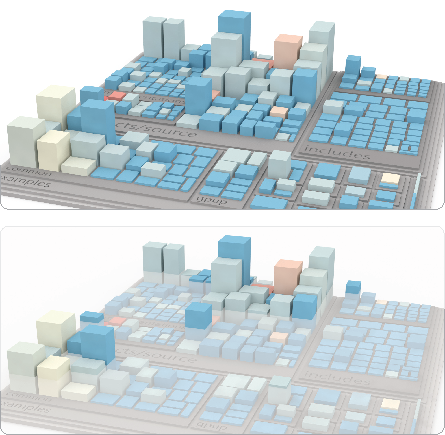
\includegraphics[width=\linewidth]{height-reference-teaser}
	\caption{A software map (top)---a 2.5D treemap depicting software system information---using a transparent plane for the visual display of height reference (bottom). A small open-source project is depicted, with the number of changes of a source code unit (color)  correlated to the number of different developers per unit (height). The height reference allows for a precise identification of error-prone code units.}
	\label{fig:teaser}
\end{figure}

\section{Introduction}
\label{sec:introduction}
\noindent A 2D treemap visualizes \emph{tree-structured data elements} (nodes) and \emph{related thematic information} (attributes) in a space-filling way~\cite{Johnson1991}, i.e., 
it maps attributes to graphical elements that are recursively stacked within their parents' elements.
The visualization technique is applied in various research and industry applications to provide a comprehensive and consistent gestalt for communication and visual analytics~\cite{MacEachren1995} of non-spatial, massive, temporal and structurally evolving information such as file systems~\cite{Shneiderman1992} or software systems~\cite{Bohnet2011}.
Furthermore, it is easy to implement and can be efficiently rendered in real-time~\cite{Fekete2002}. 

The visualization and communication capabilities of 2D treemaps are limited compared to 2.5D treemaps that feature the third dimension~\cite{Schulz2011}. 
They offer an additional dimension for extended information display---not only using height but also transparency or texture%
---and similar to 2D variants, can be efficiently rendered~\cite{Trapp2013}. 
The added value of height, however, is limited by the treemap's overall appearance as well as the available interaction metaphors:
we often find height to be either (1) reduced to a rough indication of data trends and correlations or (2) exposed to inaccurate user estimates with respect to the actual mapped values of meticulous resolution.
Furthermore, a user's height estimate might be hindered due to perspective foreshortening of cuboids, as well as occlusion (\autoref{fig:error-occlusion}) or height distorting parent node representations~\cite{Bladh2004}. 

\begin{figure}[t!] 
    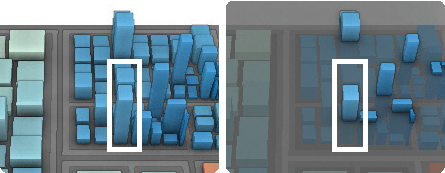
\includegraphics[width=\linewidth]{missleading-due-to-occlusion} 
	\caption{Two seemingly adjacent cuboids (outlined in white) of similar height (left). With a height reference applied a strong difference in height is exposed (right).}
    \label{fig:error-occlusion}
\end{figure} 
 
This paper introduces a \emph{height-reference technique} that enables accurate comparison of heights across the treemap and precise selection and filtering of nodes-of-interest.
For it, the following contributions are made:
\begin{itemize} 
	\item Multiple approaches for the visual display of height reference are introduced and discussed w.r.t. their applicability, usefulness, and implementation complexity.
	\item An interaction method for accurate, reference-based manipulation of the height reference within the treemap metaphor is presented.
	\item Results of a preliminary user study are presented, indicating that the use of the height reference increases accuracy for reading heights.
\end{itemize} 
\emph{Height reference} thereby denotes the depiction of a height threshold that can be interactively modified and enables height-based queries.
Within the context of this work, these details-on-demand related queries are tasks that enable accurate identification of nodes-of-interest based on their actual height. 
This comprises identification, filtering, selection, and comparison of nodes of specific, height-related characteristics:
\begin{description}
	\item [Highest Nodes]\textbar~Communication of order for identification of $n$ top-most nodes.
	\item [Similar Nodes]\textbar~Accentuation of nodes of similar or same height (peers).
	\item [Thresholded Nodes]\textbar~Exclusion or inclusion of nodes below or above a threshold respectively.
\end{description}

We argue that the introduction of an interactive height reference to 2.5D treemaps (\autoref{fig:teaser}) increases (1) accuracy of height readings, (2) allows for fast and precise identification of similar or correlating nodes, and (3) prevents miscommunication of height, e.g., caused by overlapping or occluding nodes of equally colored and shaded cuboids.
Furthermore, we show results of our prototypical implementations, provide implementation details for web-based provisioning, and, finally, present results of a preliminary study we conducted.

\section{Related Work}
\label{sec:related}
\noindent Related work includes findings in the fields of visualization of tree-structured data, interaction, as well as rendering techniques and visual quality. 
For the remainder of this work, the terminology of \emph{inclusion-based, implicit hierarchy visualization}~\cite{Schulz2011,Dubel2014} is applied.

\subsection{Treemaps} 
Treemaps were introduced as two-dimensional, space-restricted visualization of tree-structured data in 1992~\cite{Shneiderman1992} and continue to increase in number of applications and enhancements ever since. 
Often used visual variables include size and color~\cite{Fekete2002} as well as texture~\cite{Holten2005}.
Other visual variables inherent or applicable to treemaps are location, size, shape, orientation, color hue, color value, color saturation, texture, arrangement/layout/order \cite{Roth2016}.
However, we advise against the simultaneous use of more than 3 to 4 visual variables in a map theme.
For the specification of our map themes, we adhere to the information seeking mantra by mapping the most relevant attributes (for a given task) to visual variables that are subject to preattentive processing. 
The remaining visual variables are used for exploration and details-on-demand display.
In order to increase recognition of the data's topology, shading techniques~\cite{VanWijk1999} or, in our case study, margins or insets~\cite{Shneiderman1992,Lue2008} are used.
For spatialization, we use a strip inverted layout~\cite{Tu2007} and are in the transition towards hybrid, map theme and, by implication, task-aware layouting~\cite{Hahn2017hybrid}.

\subsection{2.5D Treemaps}
2.5D treemaps provide additional information display for attribute mapping by extruding the graphical elements~\cite{Bladh2004}.
The graphical elements (\emph{cuboids}) now consist of additional visual variables, e.g., height and transparency.
The spatial reference, that is the location of every graphical element, remains unchanged and the third dimension is utilized for height display only, not for 3D positioning though.
Thus, we refer to this extruded treemap as \emph{2.5D treemaps} instead of 3D treemaps~\cite{Ham2002}.

Although mapping leaf data to height is inherent, it is debatable whether or not graphical elements that represent inner nodes should have a height, e.g., depicting accumulated inner node data~\cite{Bohnet2011}.
It was suggested~\cite{Bladh2004} to increase the topological quality---a measure of the user performance and ability to read data structure, e.g., (1) associate leaf nodes to parents and (2) differentiate inner nodes by depth and adjacency---but aggravates height comparison of graphical elements of different parents and often increases the overall visual complexity.
We argue to restrict height mapping exclusively to aggregated inner nodes~\cite{Limberger2017} and increase the topological quality by an integral, well-tuned use of color schemes, contouring~\cite{Kong2010}, labeling, and margins instead.

For a comprehensive overview of variations of treemaps and similar visualization techniques, we refer to the survey by Schulz et al.~\cite{Schulz2011}.
Our height-reference technique is applicable to 2.5D visualizations such as 2.5D hierarchical edge bundles~\cite{Holten2006} and 2.5D icicle plots~\cite{Kruskal1983} as well as treemaps that limit the use of 3D to the exposition of additional detail in areas-of-interest~\cite{Chaudhuri2009,Limberger2017b}.
Such mixed uses, however, are not discussed specifically in this paper.

\begin{figure*}[!th]
	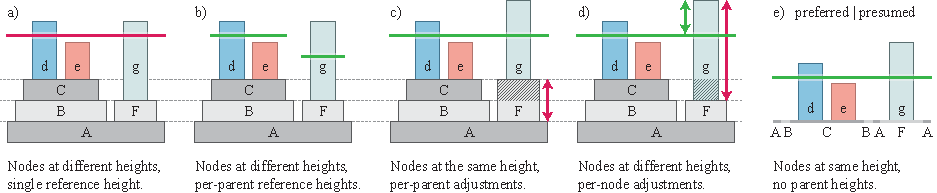
\includegraphics[width=\textwidth]{parent-height-issues}\medskip
    \caption{
        Variations of height reference for simultaneous use of cuboids for leaf and inner nodes (a to d). 
        The red and green lines suggest deceptive and genuine height readout respectively. With the virtual camera's altitude presumed to be above \ang{20}, we favor the use of overlapping or nested rectangles for inner nodes (e). 
        This reduces occlusion and visual complexity while preserving nesting clues, maintaining labeling of parents, and enabling height comparison with and without height reference.}
    \label{fig:parent-height-issues} 
\end{figure*}

\subsection{Interaction Techniques}
Interaction techniques for 2D and 2.5D treemaps typically cover navigational tasks (pan, zoom, rotate), selection and filtering tasks (e.g., implicit or explicit queries specified via GUI elements) as well as detail providing interactions (e.g., tooltips on hovering, linking cuboids to external resources).
For navigation we follow a basic world-in-hand metaphor as discussed for software maps~\cite{Limberger2013web}.
A comprehensive overview of interaction techniques was recently given by Jankowski and Hachet~\cite{Jankowski2015}.
When visualizing large data sets using treemaps, handling large numbers of graphical elements renders \emph{focus+context} and \emph{overview+detail} techniques vital for exploration~\cite{Hauser2006}.
Our height-reference technique targets big data visualization and visual analytics tasks and is intended as an auxiliary interaction technique (similar to rotation, which, in contrast to pan and zoom, is mostly used for mitigating occlusion).
With respect to the \emph{explicit height-reference}, similar techniques were presented for \enquote{cognitive aid to augment a user's ability to compare the [height] values} in 3D histograms, such as water-level metaphor or \enquote{movable baseline}~\cite{yi2007toward}. %
The various interactive prototypes that we implemented use interactive GPGPU-based rendering techniques as can be found in recent similar large data visualization techniques~\cite{Sud2010,Trapp2013}.

2.5D treemaps are limited by a number of drawbacks~\cite{Schulz2011,VanWijk2003}; occlusion, underutilized screen-space, and perspective-foreshortening problems are debated continuously in the field of thematic 3D visualization~\cite{Elmqvist2008,Roehlig2016}.
From a perceptual view, comparison of length in 3D projected geometry was found to be more difficult than it is in 2D~\cite{norman1996visual}.
Especially occlusion can lead to (1) misleading height readouts in some cases, i.e., when the junction of a leaf node's graphical element to its parent is occluded by another leaf node's element (\autoref{fig:error-occlusion}).
Miyazaki and Itoh have presented an algorithm that reduces the overlap of piles (in a pile view, comparable to cuboids in 2.5D treemaps) by means of their bounding boxes projected onto the screen~\cite{Miyazaki2009occlusion}.
This, however, is (1) not applicable to most treemap layouting algorithms \cite{Hahn2017hybrid}, (2) does not take temporal coherence on navigation into account, and (3) was only shown for a small number of piles.

In addition to occlusion, height mapping is often applied with a ludicrous data resolution, (2) exceeding the actual available pixel resolution as well as (3) overlooking the tendency of humans to overestimate the height of distant objects in comparison to objects in the foreground. %
The use of a height reference, as presented in this paper, focuses on mitigating these drawbacks while increasing the effectiveness of explorative use of 2.5D treemaps.

\section{Visual Display}
\label{sec:visual-display}
In this section, we introduce different rendering approaches for depicting the height reference within a 2.5D treemap.
To this end, we (1) state prerequisites for designing and configuring 2.5D treemaps, (2) list common requirements that should be accounted for, and, finally, (3) briefly describe the different rendering approaches.

\subsection{Prerequisites}
Due to the diversity of treemaps and their applications we made the following assumptions that should be met in order to benefit most from one of the presented rendering approaches.

\begin{itemize}
	\item We assume the height of cuboids to change only when the data or attribute mapped changes.
	Specifically, we advise against height-based filtering and selection by means of modifying the height mapping (e.g., clamping and normalizing the mapped data on the fly) in order to provide consistent cuboid heights for respective interactions.
	\item The height mapping correlates larger heights to higher relevance for any specific task.
	For example, when small or negative values are relevant for a specific task, an inverted height mapping is expected (highest node).
	\item Data outliers are handled in some form, e.g., they are removed, a non-linear mapping is used, additional visual variables are introduced, or multi-range height mapping, e.g., stacked percentiles (preferred), is used.
	\item The overall height scale is rather small to reduce occlusion and promote preattentive color processing.
	Color, weight, structure, and labeling primarily promote any given task. 
	Height and other visual variables take subordinate roles for details on demand and other subsequent, explorative queries.
\end{itemize}

A simultaneous use of cuboids for leaf and inner nodes (\autoref{fig:parent-height-issues}) should be applied with care.
In addition to increasing the occlusion and the overall visual complexity, it (1) suggests a meaningful height mapping for inner nodes---though commonly constant per node (as depicted in \autoref{fig:teaser})---and (2) aggravates height comparison even if a height reference is used. 
If not stated otherwise, the remainder of this paper assumes nested and flat (no height) parent nodes.

\subsection{Requirements}
To provide feasible means for the visual display of height references in real-time we constrained our rendering approaches to several requirements.
First of all, the rendering should not rely on transparency or translucency.
Even though it was shown that the use of transparency positively affects the perception of a visualization~\cite{jankowski2015interaction} we strive to decrease the technical needs for implementation~\cite{Enderton2011transparency} and keep the additional rendering cost to a minimum.
Transparency is especially hard to solve for even the smallest treemaps (with a few hundred overlapping cuboids) and OIT (order-independent transparency) rendering techniques either introduce visual artifacts such as noise or require lots of GPU memory or both.
Besides that, transparency might be preferred to be used as a visual variable directly already.

Parent node representations that take advantage of labeling and/or coloring should neither be fully nor partially obscured since they provide essential information regarding structural comprehension, and increase predictability of item locations within a treemap.
Even though we advise against parent heights, a rendering approach should allow for a height depiction on a per-node basis.
At best, a per-fragment based rendering would not only support cuboids, but arbitrary shapes, such as sphere maps and GPU-generated or tessellated geometry.

Finally, increasing the height threshold should reduce the overall visual complexity to facilitate spotting regions and nodes of interest.

\subsection{Rendering}
This section introduces various approaches for rendering a height reference, via intersections, an explicit surface, a closed surface, an implicit surface, stilts, and transparency bases:\medskip

\begin{wrapfigure}{l}{80pt}
    \vspace{-\baselineskip}
    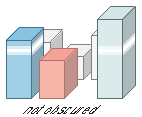
\includegraphics[width=96pt]{height-reference-intersect}
    \vspace{-1.5\baselineskip}
\end{wrapfigure}
\noindent\textbf{Intersections.}
The intersection of a surface at a height threshold is displayed using a stripe on each affected cuboid. 
Coloring might be orthogonal to the color scheme used for visual variable color, e.g., desaturate, lighten or darken.
This approach does not obscure parent nodes and also allows for identification of nodes that fall below the threshold (all cuboids without an intersection).
It is not well suited for filtering and selection though, since it hinders grouping nodes with intersections visually.\medskip

\begin{wrapfigure}{l}{80pt}
    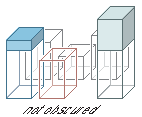
\includegraphics[width=96pt]{height-reference-stilts}
    \vspace{-1.5\baselineskip}
\end{wrapfigure}
\noindent\textbf{Stilts.}
The lower cuboid parts are cropped and replaced by one or four haloed outlines/edges (stilts) to maintain a depth cue and relation to the cuboid's location.
Even though parent nodes are not obscured, lots of overlapping lines are introduced and a cuboid's location is harder to spot.
These side effects can be reduced by rendering the lower parts transparent, but this would in turn drastically increase rendering overhead.\medskip

\begin{wrapfigure}{l}{80pt}
    \vspace{-\baselineskip}
    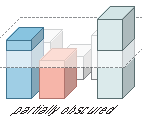
\includegraphics[width=96pt]{height-reference-explicit-surface}
    \vspace{-1.5\baselineskip}
\end{wrapfigure}
\noindent\textbf{Explicit Surface.}
A transparent plane or surface is used for depicting the height reference.
This, e.g., desaturates (depending on the blend mode used) the cuboid parts below the height threshold but also partially obscures parent nodes. 
However, depth cues imparted by screen-space based post processing---such as local ambient occlusion or unsharp-masking the depth buffer---might be decreased below the plane (and require additional rendering overhead for mitigation). 
Also, this approach cannot be easily applied node-locally nor does it account for parent heights.\medskip

\begin{wrapfigure}{l}{80pt}
    \vspace{-\baselineskip}
    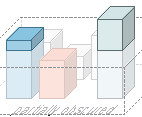
\includegraphics[width=96pt]{height-reference-closed-surface} 
    \vspace{-1.5\baselineskip}
\end{wrapfigure}
\noindent\textbf{Closed Surface.} 
Similar to the explicit surface approach, but with additional lateral surfaces down to the bottom in order to fake an infinite surface appearance.
This avoids exposure of cuboid parts below the threshold at any viewing angle, but requires the surface to seamlessly integrate with the background.\medskip

 \begin{wrapfigure}{l}{80pt}
    \vspace{-\baselineskip}
    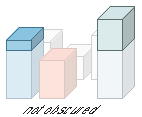
\includegraphics[width=96pt]{height-reference-implicit-surface}
    \vspace{-1.5\baselineskip}
\end{wrapfigure}
\noindent\textbf{Implicit Surface.}
All cuboids are desaturated below the height threshold on a per-fragment basis.
If applied to all cuboids, the impression of a transparent, infinite surface at the height threshold is created.
In contrast to the explicit or closed surface, parent nodes are not obscured, screen-space processing is not affected, and parent heights can be easily accounted for as well.
Similar to the intersection approach, this can also be applied for an arbitrary subset of nodes.
In any case, the overall visual display of the treemap's structure is fully preserved.
\medskip

Please note that we favor desaturation of colors in most rendering approaches in order to reduce the saliency of node representations when falling below the height threshold. 
This is, however, interchangeable with other reasonable color modifications. 
Also note that even though we promote the implicit surface (fragment-based) as the most favorable approach, explicit and closed surfaces (geometry-based) might be easier to integrate in certain visualization or rendering frameworks.
And, if more sophisticated rendering capabilities are available, these approaches can produce reasonable results (\autoref{fig:translucency-shadows}).

\begin{figure}[b]
	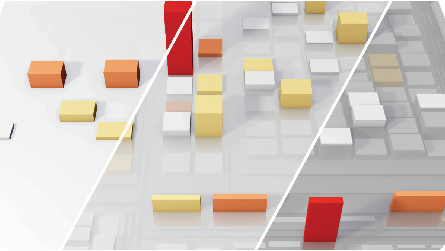
\includegraphics[width=\linewidth]{opaque-translucent-transparent}
    \caption{2.5D treemap with closed surface for height reference display using f.l.t.r. opaque, translucent, and transparent surface shading, physically based lighting, and soft shadows.}
	\label{fig:translucency-shadows} 
\end{figure}

\section{Interaction}
\label{sec:interaction}
The height reference can be denoted as a number within the domain of the attribute mapped to height.
In this section, an interaction concept for manipulating the height reference using simple point/touch or drag metaphors is presented.
A typical user interaction sequence for 2.5D treemaps can be characterized as follows:
\begin{enumerate}
    \item Gain an overview of the depicted data, understand structure, find known items or identify landmarks/nodes-of-interest.
    \item Understand the color mapping, since it is the predominant mapping and should exploit preattentive perception, i.e., locate regions-of-interest and nodes-of-interest.
    \item Only then, start exploring, e.g.,  w.r.t. the previously mentioned node characteristics (highest nodes, similar nodes, thresholded nodes).
\end{enumerate}

During exploration, the user typically uses navigation by means of pan (primary) and zoom (secondary), rotation (auxiliary, for resolving occlusion)
and pointing or picking in order to obtain additional information display of individual nodes.
For height reference manipulation we suggest introducing an additional, auxiliary picking (and subsequent drag/scroll/swipe) that behaves slightly differently based on which face of a cuboid (top or lateral) was picked initially.

\subsection{Top Cuboid Face}
If the top face of a cuboid is selected (e.g., clicked/touched) for height reference, then the height reference is set to the exact height of that cuboid.
This allows straightforward selection of nodes of equal or bigger height data.
The height reference remains unchanged until a new top face or lateral face of any cuboid is selected (\autoref{fig:interaction-top}).

\begin{figure}[!h]
    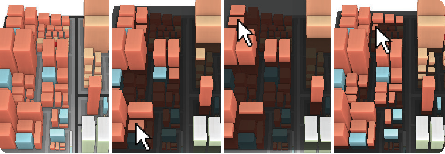
\includegraphics[width=\linewidth]{cuboid-height-interaction-top}
    \caption{A small 2.5D treemap without a height reference (left). Three unrelated mouse clicks on top faces of different nodes resulting in different height references (second to fourth subfigure).}
    \label{fig:interaction-top}
\end{figure}

\subsection{Lateral Cuboid Face}
If a lateral surface of a node's representation is selected, the picked position and the normal at this position (in case of a cuboid, the face's normal) are used to derive a virtual plane. 
The height reference is set to the height of the selected position.
For all subsequent moves (while, e.g., mouse/touch remains down) the y-coordinate of the position on the plane pointed at is used as height reference.
This allows for precise manipulation of height reference changes while being locked to the interaction's initial node.
Without this tweak, the reference height would change abruptly whenever the node pointed at changes and disrupt the exploration process (\autoref{fig:interaction-lateral}).

\begin{figure}[!h]
    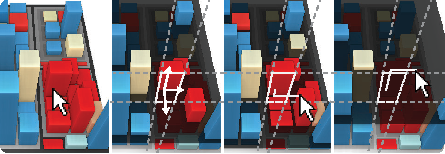
\includegraphics[width=\linewidth]{cuboid-height-interaction-lateral}
    \caption{The red node is clicked at one of its lateral faces (left). A virtual plane of all height reference values is derived (stippled lines, starting at the second subfigure). The mouse is then moved to two positions that are intersected with the plane. The height of each respective intersection point is then used as height reference (third and fourth subfigure).}
    \label{fig:interaction-lateral}
\end{figure}

\section{Preliminary User Study}
\label{sec:user-study}

We conducted a quantitative, preliminary user study in order to see if the use of a basic height reference has any benefits over not using it.
For it, we set up the following hypotheses:
\begin{description}
    \item [$H_1$] Users can identify differences in node heights faster when using the height reference (explicit surface).
    \item [$H_2$] Users can identify nodes of specific heights more accurately with the height reference (explicit surface).
\end{description}

We implemented the presented technique in a prototypical research framework (C++ and OpenGL) and applied it to 2.5D bundle views, 2.5D icicle plots, as well as 2.5D treemaps. 
We also helped integrate our technique into the WebGL-based 2.5D treemap visualization of a proprietary software analytics platform targeting mobile and desktop clients. 

For the user study, though, we used a static web interface with pseudo-interactive 2.5D treemaps featuring two specific types of interactions.
First, the 2.5D treemap could not be navigated nor manipulated except for changing the height reference by dragging to discrete, precomputed positions.
Second, three elements could be selected in order to select the three highest nodes.

Each participant was introduced to test runs for each type of question in order to understand the interactions that are available.
This was intended to reduce learning effects caused by unfamiliar interaction concepts.
The study was comprised of two different tasks, each with and without the use of our height reference.
The first task was to pick the nodes whose height was most similar to the height of a preselected node (\autoref{fig:user-study-example}).
The second task asked for identification of the three highest nodes within the whole treemap.
For each task, the time was measured.

\medskip
\noindent
The study was conducted with 20 participants with the following results:
\begin{figure}[!h]
    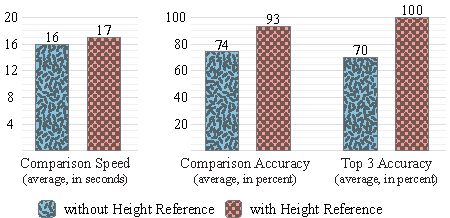
\includegraphics[width=\linewidth]{user-study-results} 
    \label{fig:user-study-results}
\end{figure}

\textbf{Speed.} We could not confirm our first hypothesis $H_1$.
The average time to respond for each task was slightly faster without the use of the height reference.\medskip

\textbf{Accuracy.} We can, however, confirm our second hypothesis $H_2$.
The use of the height reference increased the accuracy by 25\% (similar nodes) to 42\% (top 3 nodes) over the tasks completed without height reference.\bigskip

\noindent These preliminary results indicate that height-based filtering might increase the accuracy of basic height-related tasks while introducing only a marginal interaction overhead. 

\begin{figure}[t]
    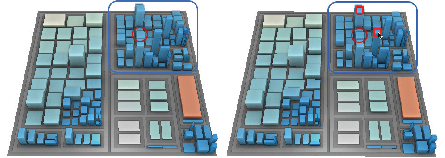
\includegraphics[width=\linewidth]{user-study-example}
    \caption{Initial treemap with preselected node circled red (left). Two user picks (nearest nodes) outlined red (right).}
    \label{fig:user-study-example}
\end{figure}

\section{Conclusion and Future Work}
\label{sec:conclusion}

This paper shows how 2.5D treemaps can be extended by an interactive, height-based filtering technique that facilitates accurate identification of highest nodes as well as similar nodes w.r.t. a height reference.
It allows filtering and selection of nodes based on their height and depicts filtered and unselected nodes in a clean way without introducing additional visual clutter.
For the rendering, various techniques are introduced and compared by means of technical needs, partial obscuration of structural information, visual complexity, and flexibility.
The fragment-based visual display of height reference using an implicit surface is preferred since it can be implemented on a node-local basis and does not assume a specific shape of the node, as long as it supports the visual variable height. 
It can be applied not only for 2.5D treemaps, but for spheremaps, 2.5D icicle plots, 2.5D circular bundle views and similar visualization techniques.

A full quantitative user study that investigates the impact of 2.5D treemap navigation metaphors mixed with the use of the presented interactive height-reference manipulation is missing and the visual quality of the various rendering approaches could be further quantified.
Finally, we would like to further investigate the benefit of our technique when depicting massive amounts of data using dynamically aggregated treemaps since we expect an increase in interaction speed as well when depicting hundreds of thousands of nodes.

\begin{acks}
The authors would like to thank Jonathan Herdt, Christoph Keßler, and Jan-Tobias Matysik for their preceding prototypes and valuable contributions.
\end{acks}

\balance
\bibliographystyle{ACM-Reference-Format}
\bibliography{references}

\end{document}
